
%(BEGIN_QUESTION)
% Copyright 2006, Tony R. Kuphaldt, released under the Creative Commons Attribution License (v 1.0)
% This means you may do almost anything with this work of mine, so long as you give me proper credit

How much pressure is being applied to this U-tube water manometer, in units of ``inches of water column'' and ``pounds per square inch''?

$$\includegraphics[width=15.5cm]{i00162x01.eps}$$

\underbar{file i00162}
%(END_QUESTION)





%(BEGIN_ANSWER)

Applied pressure = 3.1875 "W.C., which is equal to 0.1152 PSI.

\vskip 10pt

Follow-up question: demonstrate how we could have arrived at an approximate answer by using rounded figures for our unit-conversion constants, and ``mental math'' instead of a calculator.

%(END_ANSWER)





%(BEGIN_NOTES)


%INDEX% Measurement, pressure: manometer

%(END_NOTES)


